\documentclass[12pt, twoside]{article}
\usepackage[letterpaper, margin=1in, head=30pt, headsep=0.1in]{geometry}
\usepackage[english]{babel}
\usepackage[utf8]{inputenc}
\usepackage{amsmath}
\usepackage{amsfonts}
\usepackage{amssymb}
\usepackage{tikz}
\usetikzlibrary{quotes, angles}

\usepackage{graphicx}
\usepackage{enumitem}
\usepackage{multicol}

%\usepackage{pgfplots}
%\pgfplotsset{width=10cm,compat=1.9}
%\usepgfplotslibrary{statistics}
%\usepackage{pgfplotstable}
%\usepackage{tkz-fct}
%\usepackage{venndiagram}

\usepackage{fancyhdr}
\pagestyle{fancy}
\fancyhf{}
\renewcommand{\headrulewidth}{0pt} % disable the underline of the header
\raggedbottom
\newif\ifmeta
\metatrue %print standards and topics tags

\title{High School Geometry problem sets}
\author{Chris Huson}
\date{March 2021}

%\fancyhead[RE]{\thepage}
%\fancyhead[RO]{\thepage \\ Name: \hspace{3cm}}
%\fancyhead[L]{BECA / Dr. Huson / 10th Grade Geometry\\* 7 June 2019}
%
%\begin{document}
%\subsubsection*{13.7 Homework: Cross sections, distance applications}
%\fancyhead[L]{BECA / Dr. Huson / Geometry 03-Volume+angle-bisectors\\* pset ID: 34}

\begin{document}

\subsubsection*{6.16 Exam: Slope and linear equations\\
\emph{You must show the values substituted in the formula} for credit. Optional: Graspable Math, Geogebra}
\begin{enumerate}
\item Plot the points and the line $\overleftrightarrow{PQ}$, $P(1,3)$, $Q(4,5)$. Calculate its slope:
  \begin{multicols}{2}
  $\displaystyle m = \frac{y_Q - y_P}{x_Q - x_P}$
    \vspace{2cm}
    \begin{flushright}
    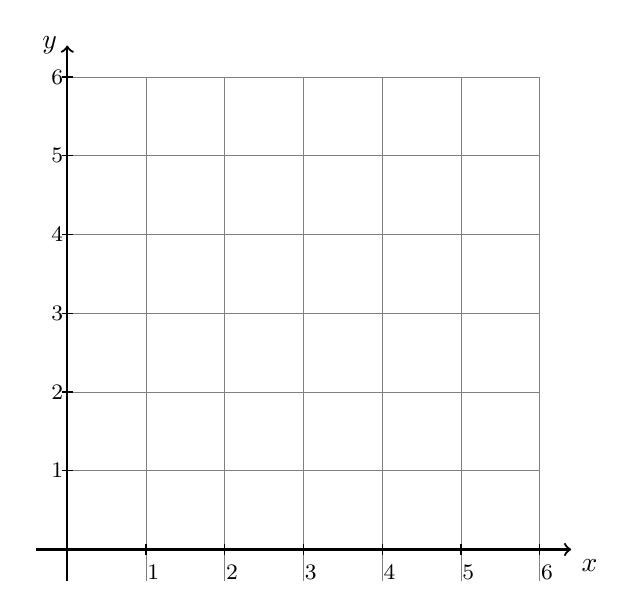
\begin{tikzpicture}[scale=1]
      \draw [help lines] (0,-0.4) grid (6,6);
      \draw [thick, ->] (-0.4,0) -- (6.4,0) node [below right] {$x$};
      \foreach \x in {1,2,3,4,5,6}
        \draw[shift={(\x,0)},color=black] (0pt,2pt) -- (0pt,-2pt) node[below] {\footnotesize \; $\x$};
      \draw [thick, ->] (0,-0.4)--(0,6.4) node [left] {$y$};
      \foreach \y in {1,2,3,4,5,6}
        \draw[shift={(0,\y)},color=black] (-2pt,0pt) -- (2pt,0pt) node[left] {\footnotesize \; $\y$};
      %\draw [fill] (2,1) circle [radius=0.05] node[above left] {$A(2,1)$};
      %\draw [fill] (3,4) circle [radius=0.05] node[above right] {$B(3,4)$};
      %\draw [<->, thick] (1,-2)--(4,7);
    \end{tikzpicture}
    \end{flushright}
    %https://graspablemath.com/canvas?load=_3049ffb53f2793d5
\end{multicols}

\newpage  
\item Find the slope of the line $\overleftrightarrow{AB}$, $A(13,2.2)$, $B(57,3.3)$. Express the value as a percent (the percent grade).
    \begin{flushright}
      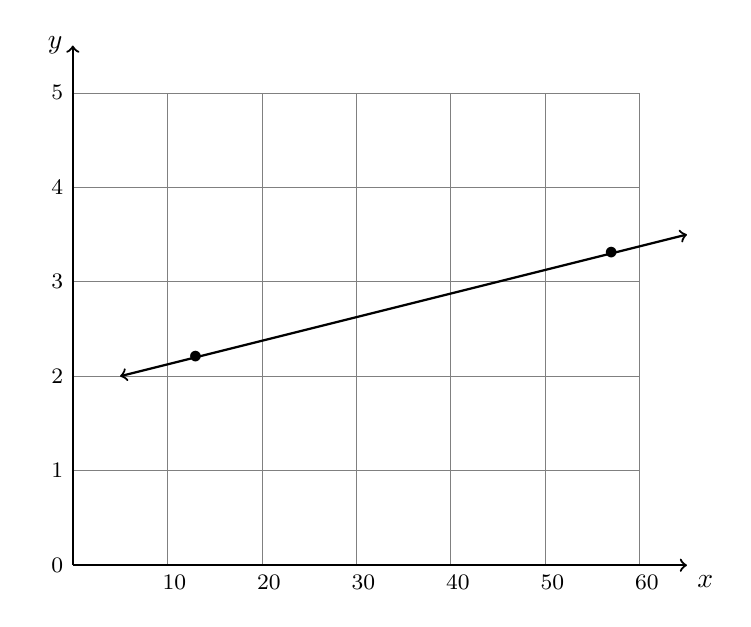
\begin{tikzpicture}[xscale=0.12, yscale=1.2]
        \draw [help lines, xstep=10, ystep=1] (0,0) grid (60,5);
        \draw [thick, ->] (0,0) -- (65,0) node [below right] {$x$};
        \foreach \x in {10,20,...,60}
          \draw[shift={(\x,0)},color=black] (0pt,0pt) -- (0pt,0pt) node[below] {\footnotesize \; $\x$};
        \draw [thick, ->] (0,0)--(0,5.5) node [left] {$y$};
        \foreach \y in {0,1,...,5}
          \draw[shift={(0,\y)},color=black] (0pt,0pt) -- (0pt,0pt) node[left] {\footnotesize \; $\y$};
        \node at (13,2.2) {$\bullet$};
        \node at (57,3.3) {$\bullet$};
        %\draw [fill] (3,4) circle [radius=0.05] node[above right] {$B(3,4)$};
        \draw [<->, thick] (5,2.0)--(65,3.5);
      \end{tikzpicture}\\
      \emph{Not to scale}
      %https://graspablemath.com/canvas?load=_80dee8e691bb7193
      \end{flushright}

\newpage
\item Find the slope (or ``grade'') for a six inch rise over a run of $12 \frac{1}{2}$ feet.
\begin{multicols}{2}
  Express your result as follows: 
\begin{enumerate}
  \item Fraction
  \item Decimal
  \item Percentage
\end{enumerate}
\begin{flushright}
  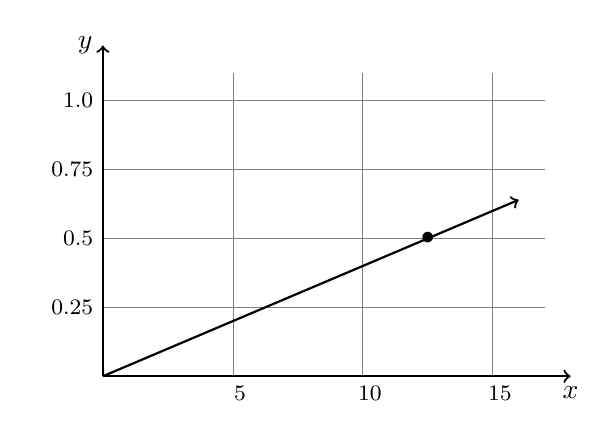
\begin{tikzpicture}[xscale=0.33, yscale=3.5]
    \draw [help lines, xstep=5, ystep=0.25] (0,0) grid (17,1.1);
    \draw [thick, ->] (0,0) -- (18,0) node [below] {$x$};
    \foreach \x in {5,10,15}
      \draw[shift={(\x,0)},color=black] (0pt,0pt) -- (0pt,0pt) node[below] {\footnotesize \; $\x$};
    \draw [thick, ->] (0,0)--(0,1.2) node [left] {$y$};
    \foreach \y in {0.25, 0.5, 0.75, 1.0}
      \draw[shift={(0,\y)},color=black] (0pt,0pt) -- (0pt,0pt) node[left] {\footnotesize \; $\y$};
    \node at (12.5,0.5) {$\bullet$};
    %\draw [fill] (3,4) circle [radius=0.05] node[above right] {$B(3,4)$};
    \draw [->, thick] (0,0)--(16,0.64);
  \end{tikzpicture}
  \emph{Not to scale}
\end{flushright}
%https://graspablemath.com/canvas?load=_6bf89509a6863ef1
\end{multicols}

\newpage
\item Complete each statement about linear equations.
\begin{enumerate}[itemsep=0.5cm]
  \item What is the $y$-intercept of the line $y = 0.75x - 1.25$?
  \item What is the slope of a vertical line?
  \item What is the percent grade of the line $\displaystyle y = 0.035x + 5.0$?
  \item What is the slope of the line $y=\frac{1}{2}$?
  \item If $m = 0.75$ then $m_{\perp}=$
  \item Lines $p$ and $q$ have slopes $m_p = -5$ then $m_q= 0.20$. Are they parallel, perpendicular, or neither? Justify your answer by showing the product of their slopes.
  \end{enumerate}

\newpage  
\item Find the equation of the line through the points $(0,1.2)$, $(50,3.7)$. First find the slope, then substitute the slope and $y$-intercept into a linear equation.
\begin{multicols}{2}
  $\displaystyle m = \frac{y_2 - y_1}{x_2 - x_1}$, \hspace{1cm} $y=mx+b$
  \columnbreak
  \begin{flushright}
    \emph{Not to scale}\\
    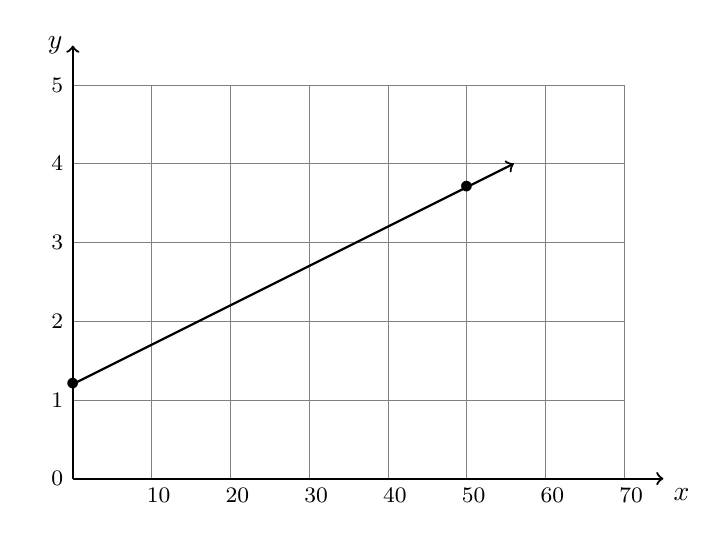
\begin{tikzpicture}[xscale=0.1, yscale=1]
      \draw [help lines, xstep=10, ystep=1] (0,0) grid (70,5);
      \draw [thick, ->] (0,0) -- (75,0) node [below right] {$x$};
      \foreach \x in {10,20,...,70}
        \draw[shift={(\x,0)},color=black] (0pt,0pt) -- (0pt,0pt) node[below] {\footnotesize \; $\x$};
      \draw [thick, ->] (0,0)--(0,5.5) node [left] {$y$};
      \foreach \y in {0,1,...,5}
        \draw[shift={(0,\y)},color=black] (0pt,0pt) -- (0pt,0pt) node[left] {\footnotesize \; $\y$};
      \node at (0,1.2) {$\bullet$};
      \node at (50,3.7) {$\bullet$};
      %\draw [fill] (3,4) circle [radius=0.05] node[above right] {$B(3,4)$};
      \draw [->, thick] (0,1.2)--(56,4.0);
    \end{tikzpicture}
    https://graspablemath.com/canvas?load=\_76c51984e075c2c2 %note underbar escape
    \end{flushright}
  \end{multicols}

\newpage
\item Is the point $P(55,3.6)$ on the line: $y=0.04x+1.40$? \\[0.5cm]
Support your answer algebraically (substitute $P$'s coordinates into the equation).
\begin{flushright}
  \emph{Not to scale}\\
  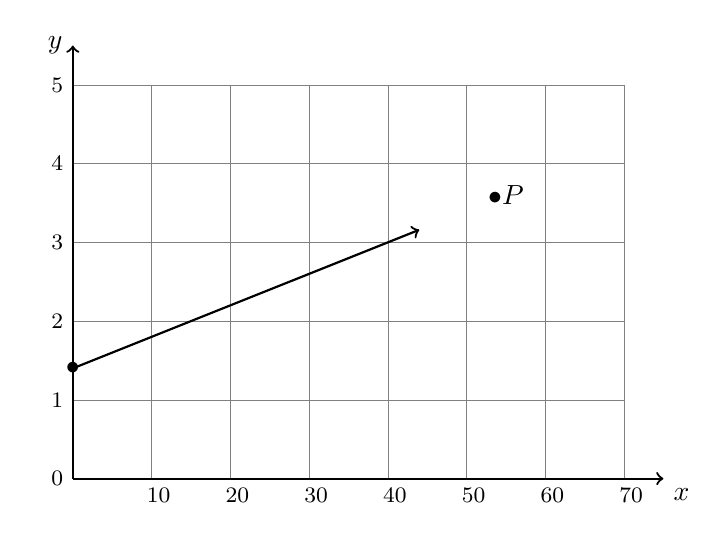
\begin{tikzpicture}[xscale=0.1, yscale=1]
    \draw [help lines, xstep=10, ystep=1] (0,0) grid (70,5);
    \draw [thick, ->] (0,0) -- (75,0) node [below right] {$x$};
    \foreach \x in {10,20,...,70}
      \draw[shift={(\x,0)},color=black] (0pt,0pt) -- (0pt,0pt) node[below] {\footnotesize \; $\x$};
    \draw [thick, ->] (0,0)--(0,5.5) node [left] {$y$};
    \foreach \y in {0,1,...,5}
      \draw[shift={(0,\y)},color=black] (0pt,0pt) -- (0pt,0pt) node[left] {\footnotesize \; $\y$};
    \node at (0,1.4) {$\bullet$};
    \node at (55,3.6) {$\bullet P$};
    %\draw [fill] (3,4) circle [radius=0.05] node[above right] {$B(3,4)$};
    \draw [->, thick] (0,1.4)--(44,3.16);
  \end{tikzpicture}
  https://graspablemath.com/canvas?load=\_ecee681f9b231be0
  %https://graspablemath.com/canvas?load=_ecee681f9b231be0
  \end{flushright}

\newpage
\item Quadrilateral $ABCD$ with vertices $A(3,7)$, $B(-1,1)$, $C(2,-1)$, and $D(6,5)$ is shown. \\[0.5cm]
Write down the slopes of each side.
\begin{multicols}{2}
  Slope of $\overline{AB}=$\\[0.8cm]
  Slope of $\overline{BC}=$\\[0.8cm]
  Slope of $\overline{CD}=$\\[0.8cm]
  Slope of $\overline{AD}=$\\[0.8cm]
  Is $ABCD$ a parallelogram? \\[0.8cm]
  Is it a rectangle? \\[0.8cm]
  Justify your answers below, citing the slopes and their relationships.
  \begin{flushright}
    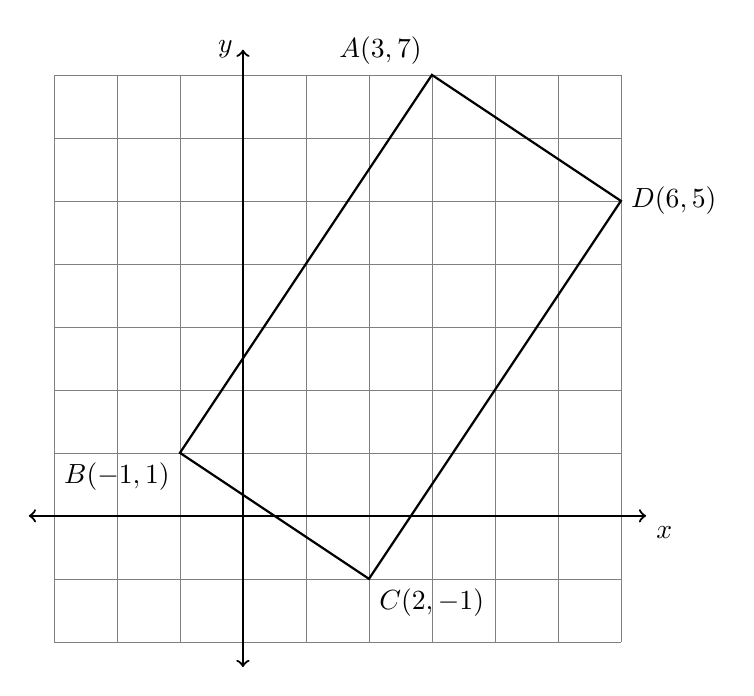
\begin{tikzpicture}[scale=0.8]
      \draw [help lines] (-3,-2) grid (6,7);
      \draw [thick, <->] (-3.4,0) -- (6.4,0) node [below right] {$x$};
      \draw [thick, <->] (0,-2.4)--(0,7.4) node [left] {$y$};
      \draw [thick] (3,7) node[above left] {$A(3,7)$}--
        (6,5) node[right] {$D(6,5)$}--
        (2,-1) node[below right] {$C(2,-1)$}--
        (-1,1) node[below left] {$B(-1,1)$}--
        cycle;
    \end{tikzpicture}
    \end{flushright}
  \end{multicols}

\newpage 
\item Plot a parallelogram (not a rectangle) using Geogebra (use the grid). The legs must not be horizontal or vertical. Paste an image of your work in this Classkick slide from the clipboard or by using the ``camera'' tool.\\[0.25cm]
Spicy: Show the measures the slopes of the quadrilateral sides.

\newpage
\item A line through the point $A(2,2)$ has a $y$-intercept of 6. 
\begin{enumerate}
  \item Write down the equation of the line.
  \item What slope is perpendicular to the line?
  \item Spicy: What is the equation of the perpendicular line through $A$?
\end{enumerate}
\begin{flushright}
  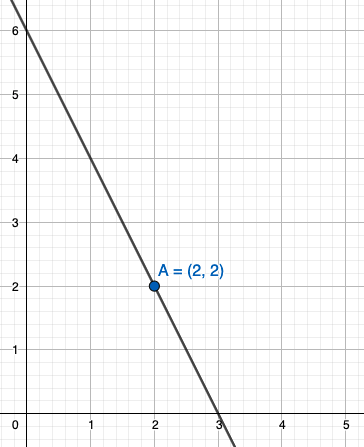
\includegraphics[width=8cm]{6-16-9-perpendicular.png}
%https://graspablemath.com/canvas?load=_2e1c5526e6f2c45c
\end{flushright}

\newpage
\item Given $\triangle ABC$ as shown with $A(0,6)$, $B(3,4)$, $C(1,1)$.
\item \begin{multicols}{2}
  \begin{enumerate}
    \item Write down the equation of $\overleftrightarrow{AB}$.
    \item Write the equation of line $\overleftrightarrow{BC}$.
    \item Is $\overleftrightarrow{AB} \perp \overleftrightarrow{BC}$? \\[1cm]
    Show the product of their slopes is or is not $-1$. \\[3cm]
    \end{enumerate}
\columnbreak
    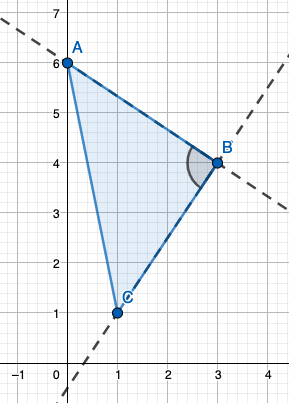
\includegraphics[width=7.5cm]{6-16-10-triangle.png}
    https://www.geogebra.org/calculator/myk4wwbj
\end{multicols}


\end{enumerate}
\end{document}